\documentclass[tikz,border=7pt]{standalone}
\usepackage{amsmath,amssymb}
\usetikzlibrary{arrows.meta,patterns,decorations.markings,calc}
\tikzset{outline/.style={line width=.7pt,line cap=round,line join=round},
 map/.style={outline,-{Stealth[length=2.1mm,width=1.5mm]}},
 point/.style={circle,draw,fill=white,inner sep=1.4pt,line width=.6pt},
 along/.style={postaction={decorate},decoration={markings,mark=at position .52 with {\arrow{Stealth[length=1.8mm,width=1.2mm]}}}}}
\begin{document}
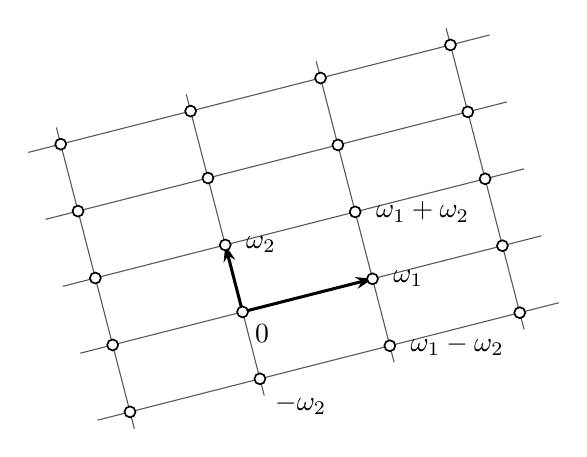
\begin{tikzpicture}[font=\normalsize]

\begin{scope}[x={(1.65cm,.42cm)},y={(-.22cm,.85cm)}]
\foreach \j in {-1,...,3}{\draw[line width=.4pt,black!65] (-1.25,\j)--(2.3,\j);}
\foreach \i in {-1,...,2}{\draw[line width=.4pt,black!65] (\i,-1.25)--(\i,3.25);}
\draw[map,line width=1.1pt] (0,0)--(1,0);
\draw[map,line width=1.1pt] (0,0)--(0,1);
\foreach \i in {-1,...,2}{\foreach \j in {-1,...,3}{\node[point] at (\i,\j) {};}}
\node[below right=1pt] at (0,0) {$0$};
\node[right=4pt] at (1,0) {$\omega_1$};
\node[right=4pt] at (0,1) {$\omega_2$};
\node[right=4pt] at (1,1) {$\omega_1+\omega_2$};
\node[below right=2pt] at (0,-1) {$-\omega_2$};
\node[right=4pt] at (1,-1) {$\omega_1-\omega_2$};
\end{scope}

\end{tikzpicture}
\end{document}
